\section{Theory and Technical Background}
\label{sec:theory-and-technical-background}
To achieve ultrasonic distance
measurement, the main components we use are the HC-SR04 ultrasonic distance
measurement module and the SG90 servo motor.

The HC-SR04 (Figure~\ref{fig:hc-sr04}) ultrasonic distance measurement module consists of an ultrasonic transmitter and a receiver.
The transmitter sends ultrasonic waves in a specific direction.
When the ultrasonic waves encounter an obstacle, they are reflected back, and the receiver captures the reflected waves.
By calculating the time difference between the emission and reception of the ultrasonic waves, combined with the speed of sound, the distance can be determined.
When the ultrasonic wave is emitted, the Echo pin becomes high.
When the ultrasonic wave is received by the receiver, the Echo pin becomes low.
By measuring the duration of the high state of the Echo pin, the time of ultrasonic wave propagation can be obtained.

\begin{figure}[H]
  \centering
  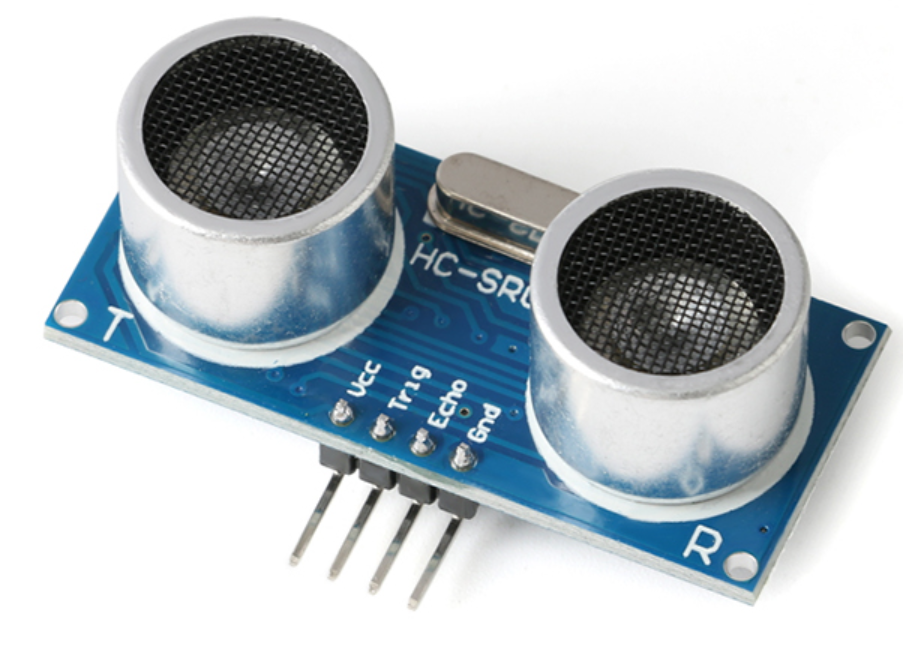
\includegraphics[width=0.6\linewidth]{Figures/HC-SR04}
  \rule{35em}{0.5pt}
  \caption{HC-SR04 ultrasonic distance measurement module}
  \label{fig:hc-sr04}
\end{figure}

The SG90 (Figure~\ref{fig:sg90}) servo motor is a position (angle) servo driver, suitable for control systems that
require continuous angle changes and the ability to maintain a specific angle.
It is mainly composed of a casing, circuit board, DC motor, gear reduction set,
and position detection element (control circuit), forming an automatic (closed-loop) control device.

\begin{figure}[H]
  \centering
  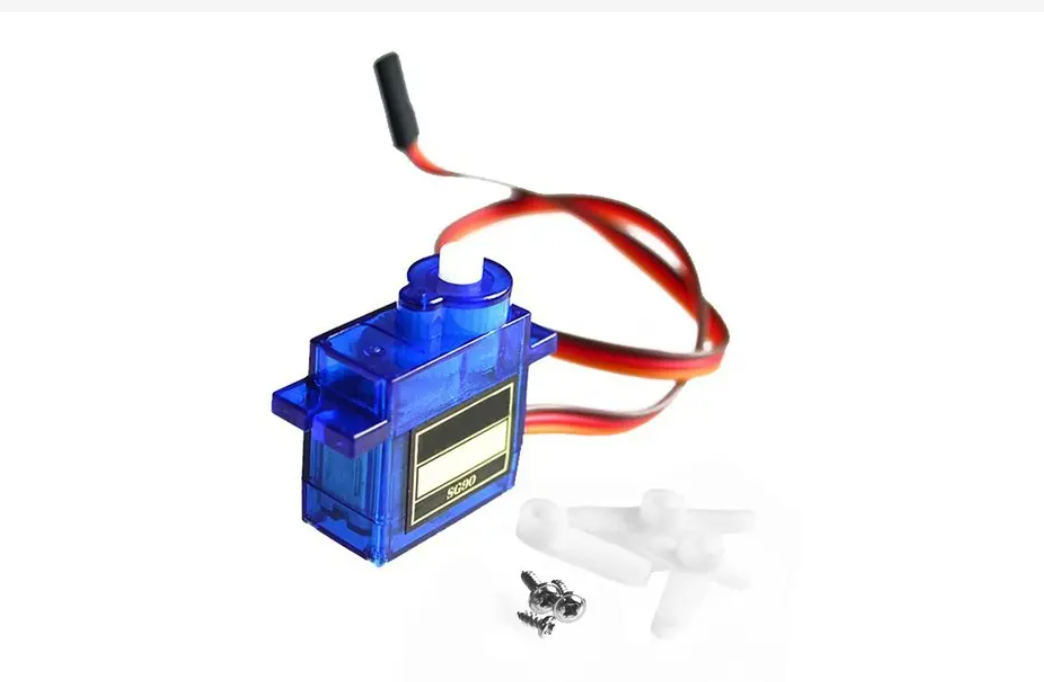
\includegraphics[width=0.6\linewidth]{Figures/SG90}
  \rule{35em}{0.5pt}
  \caption{SG90 servo motor}
  \label{fig:sg90}
\end{figure}
